%Set the document class we will be using.
%We do not need anything special, so I go with article
\documentclass[]{article}

%Now, we can import whatever packages we may need
%These are the ones I commonly utilize.
\usepackage{amsmath} %Contains useful commands like \text and equation environment
\usepackage{amsthm} %Helps to define theorem structures, includes \newtheorem and proof environment
\usepackage{amssymb} %Provides an extended symbol collection
\usepackage{graphicx} %Allows us to display figures
\usepackage{fancyvrb} %Contains the Verbatim environment, allowing us to type code blocks
\usepackage{fancyhdr} %Allows us to customize headers and footers
\usepackage{lastpage} %Gives us the last page as a command \pageref{LastPage}
\usepackage{hyperref} %Allows us to have hyper links in our text
\usepackage{pgfplots} %Allows us to make beautiful graph and plots
\pgfplotsset{compat=1.18} %Puts pgfplots into proper compatibility for this version of latex

%Here we create some useful shortcuts for fancy characters and spacing
\newcommand{\bb}[1]{\mathbb{#1}} %Shortcut for bold faced characters
\newcommand{\Z}{\bb{Z}} %Returns the set of Integers symbol
\newcommand{\Q}{\bb{Q}} %Returns set of rational numbers symbol
\newcommand{\R}{\bb{R}} %Real numbers symbol
\newcommand{\C}{\bb{C}} %Complex numbers symbol
\newcommand{\N}{\bb{N}} %Natural numbers symbol
\newcommand{\dent}{\hspace{\parindent}} %Forces an indent in the current line

%Adjust our page setup
\setlength{\topmargin}{-0.3in} %Removes some top margin so our header and footer begins higher up
\setlength{\oddsidemargin}{0in} %Custom margin for even and odd pages
\setlength{\evensidemargin}{0in} %Used when printing double-sided papers 
\setlength{\textheight}{9in} %Leaves 1 inch at top and 1 inch at bottom
\setlength{\textwidth}{6.5in} %Leaves 3/4 inch on each side
\setlength{\parindent}{20pt} %Here you can customize a paragraph indentation

%Set up our headers and footers
\pagestyle{fancy} %Sets our page style using fancyhdr
\lhead{The Hitchhiker's Guide to LaTeX} %Left Header
\rhead{Stephen Lasinis} %Right Header
\cfoot{\thepage \ of \pageref{LastPage}} %Center Footer
\renewcommand{\footrulewidth}{0.4pt} %Enables horizontal line above the footer

%Set up our hyperlink settings
\hypersetup{colorlinks, citecolor=black, filecolor=black, linkcolor=black, urlcolor=blue}


\begin{document}

    \begin{titlepage}
        \begin{center}
        
            \vspace{3in}

            \LARGE
            \textbf{The Hitchhiker's Guide to LaTeX}

            \vspace{0.1in}

            \normalsize
            An Aid in Writing Math Homework

            \vspace{1in}

            \large
            \textbf{Stephen Lasinis}

            \vspace{0.2cm}

            \normalsize
            slasinis@uwm.edu
            
            \vfill

            \normalsize
            
            \vspace{0.2in}

            
\includegraphics[width=2in]{uwm.png}

            \vspace{0.25in}

            University of Wisconsin - Milwaukee
        \end{center}
    \end{titlepage}

    \newpage

    \tableofcontents

    \newpage

    \section{Packages}
    \dent Below is a list of staple packages to use when creating a document as well as a link to their documentation. The most useful contents of these packages will be described later, in more detail. If you attempt to use a command or an environment without importing the proper package, \textbf{Overleaf} will tell you which package is required; this way, you do not have to memorize what each package contains. Instead, you are able to focus on the specific commands and environments you will need. These packages can be imported into your document with the use of the following command:
    \begin{verbatim}
        \usepackage{packagename}
    \end{verbatim}
    \begin{itemize}
        \item amsmath \\
        The \textbf{amsmath} package user's guide can be found \href{http://www.ams.org/arc/tex/amsmath/amsldoc.pdf}{\textbf{here}}.

        \item amsthm \\
        The \textbf{amsthm} package user's guide can be found \href{http://www.ams.org/arc/tex/amscls/amsthdoc.pdf}{\textbf{here}}.

        \item amssymb \\
        The \textbf{amssymb} package reference sheet can be found \href{https://milde.users.sourceforge.net/LUCR/Math/mathpackages/amssymb-symbols.pdf}{\textbf{here}}.

        \item graphicx \\
        A guide to using the \textbf{graphicx} package write-up  can be viewed \href{https://www.kwasan.kyoto-u.ac.jp/solarb6/usinggraphicx.pdf}{\textbf{here}}.

        \item fancyvrb \\
        A guide to using the \textbf{fancyvrb} package can be viewed \href{https://texdoc.org/serve/fancyvrb/0}{\textbf{here}}.

        \item fancyhdr \\
        Information regarding the usage of \textbf{fancyhdr}, as well as basic header and footer elements can be found \href{https://www.overleaf.com/learn/latex/Headers_and_footers}{\textbf{here}}.

        \item lastpage \\
        Information about the \textbf{lastpage} package can be viewed \href{https://ctan.mirror.garr.it/mirrors/ctan/macros/latex/contrib/lastpage/lastpage.pdf}{\textbf{here}}.

        \item hyperref \\
        The \textbf{hyperref} package write-up can be view on \href{https://www.overleaf.com/learn/latex/Hyperlinks}{\textbf{Overleaf}}.

        \item pgfplots \\
        The full documentation for \textbf{pgfplots} can be found \href{https://www.iro.umontreal.ca/~simardr/pgfplots.pdf}{\textbf{here}}.
        
    \end{itemize}

    \section{Document Sectioning}
    \subsection{Overview}
    \dent Documents usually follow some type of logical structure (i.e. chapters, sections, parts, etc.). LaTeX has 7 levels of depth for defining sections:
    \begin{verbatim}
        \part{part}
        \chapter{chapter}
        \section{section}
        \subsection{subsection}
        \subsubsection{subsubsection}
        \paragraph{paragraph}
        \subparagraph{subpragraph}
    \end{verbatim}
    Typically, \textbf{$\backslash$section} is the highest level a given document will need, especially in regards to homework.
    \newpage
    \subsection{Numbered and Unnumbered Sections Syntax}
    \dent The syntax for a numbered section:
    \begin{verbatim}
        \section{section}
        \subsection{subsection}
        ...
    \end{verbatim}
    The syntax for an unnumbered section:
    \begin{verbatim}
        \section*{section}
        \subsection*{subsection}
        ...
    \end{verbatim}

    \section{Symbols and Equations}
    \subsection{Introduction}
    This section will demonstrate how to create symbols, mix text with equations, and use the equation environment.
    \subsection{Inline Equations}
    \dent Suppose we are writing a paragraph of text and it is necessary to include a formula or variable definition within the paragraph. The following is an example syntax:
    \begin{verbatim}
        Suppose we want to define a variable in this paragraph. We would type: Let $a=5$
        or \(a=5\) where the double dollar signs encase an equation in math mode. Within 
        math mode, the user has access to various symbols and greek letters, such as 
        $\alpha,\beta,\gamma \in \Z$. You can also perform an inline equation with 
        \[ \alpha \cdot \beta = \varepsilon \] where everything between the brackets is 
        in math mode.These equations are unnumbered.
    \end{verbatim}
    Compiling the above text results in: \\
    \dent Suppose we want to define a variable in this paragraph. We would type: Let $a=5$ or \(a=5\) where the double dollar signs encase an equation in math mode. Within math mode, the user has access to various symbols and Greek letters, such as $\alpha,\beta,\gamma \in \Z$. You can also perform an inline equation with \[ \alpha \cdot \beta = \varepsilon \] where everything between the brackets is in math mode and is given its own line. These equations are unnumbered.
    \subsection{Equation Environment}
    This section will give the example syntax for a numbered equation, as well as an unnumbered equation using the equation environment. The following is an example of a numbered equation:
    \begin{verbatim}
        \begin{equation}
            \Gamma(n) = \int_{0}^{\infty} t^{z-1}e^{-t}dt
        \end{equation}
    \end{verbatim}
    After compiling, it looks like this:
    \begin{equation}
        \Gamma(n) = \int_{0}^{\infty} t^{z-1}e^{-t}dt
    \end{equation}
    As you can see, the former equation has also been labeled (1). This makes it easy to reference later in the document. The following is an example of the same equation, but unnumbered:
    \begin{verbatim}
        \begin{equation*}
            \Gamma(n) = \int_{0}^{\infty} t^{z-1}e^{-t}dt
        \end{equation*}
    \end{verbatim}
    Compiling yields the following:
    \begin{equation*}
        \Gamma(n) = \int_{0}^{\infty} t^{z-1}e^{-t}dt
    \end{equation*}
    Notice the only difference between the two environments is the asterisk following the word equation.
    \subsection{Subscripts, Superscripts, and Parentheses}
    In order to write the equations seen above, you must know how to display subscripts and superscripts. The following is an example of what you would write:
    \begin{verbatim}
        In order to get subscripts, after a symbol, place an underscore like $a_{i}$.\\
        To get a superscript, simple place a carrot after the symbol like $a^{2}$.\\
        If you need to combine them after the same symbol, yuo do so as $a_{ij}^{2}$.
    \end{verbatim}
    The following compiles to appear as: \\
    In order to get subscripts, after a symbol, place an underscore like $a_{i}$.\\
    To get a superscript, simple place a carrot after the symbol like $a^{2}$.\\
    If you need to combine them after the same symbol, you do so as $a_{ij}^{2}$. \\ \\
    The following is an example of how to create fractions:
    \begin{verbatim}
        \alpha = (\frac{\frac{a+c}{b+d}}{ab+cd})
    \end{verbatim}
    This appears as \[\alpha = (\frac{\frac{a+c}{b+d}}{ab+cd})\] You'll notice the parentheses do not scale with the height of the equation. The following is a fix for that:
    \begin{verbatim}
        \alpha = \left( \frac{\frac{a+c}{b+d}}{ab+cd} \right)
    \end{verbatim}
    This compiles as \[\alpha = \left( \frac{\frac{a+c}{b+d}}{ab+cd} \right)\] by utilizing the $\backslash$left and $\backslash$right followed by a parenthesis to scale the parentheses to scale with anything inside.

    \section{Lists and Enumerations}
    \subsection{Overview}
    \dent Lists and enumerations are perfect for when you have numbered problems or other various lists that need to be organized. In the following sections are examples of how to use the list and itemize environments.
    \subsection{Enumerate Environment}
    The enumerate environment allows the user to create an ordered list. The following is the syntax for creating an enumeration:
    \begin{verbatim}
        \begin{enumerate}
            \item This is the first item \\
            This is more text on a new line using $\backslash \backslash$
            \item This is the second item \\
            Notice the numbering is automatic.
        \end{enumerate}
    \end{verbatim}
    The code above produces the following result:
    \begin{enumerate}
        \item This is the first item \\
        This is more text on a new line using $\backslash \backslash$
        \item This is the second item \\
        Notice the numbering is automatic.
    \end{enumerate}
    \subsection{Itemize Environment}
    The itemize environment allows the user to create a list with custom item labels. The following is an example of the syntax for creating an itemize list:
    \begin{verbatim}
        \begin{itemize}
            \item[1.] This is the first item.
            \item[(a)] This is the second item.
            \item[!] This is another example.
        \end{itemize}
    \end{verbatim}
    The code above produces the following:
    \begin{itemize}
        \item[1.] This is the first item.
        \item[(a)] This is the second item, but instead of a number, we use the letter (a).
        \item[!] This is another example.
    \end{itemize}

    \section{Proofs}
    \dent The following is an example use of the proof environment:
    \begin{verbatim}
        \begin{proof}
            Let $\sigma,\tau,\mu \in S_n$. Assume $\sigma \circ \tau = \sigma \circ \mu$. 
            We want to show that $\tau = \mu$. Using the group properties for $S_n$ from 
            \textbf{Section 6.2}, we know $\sigma$ has an inverse element, 
            $\sigma^{-1} \in S_n$, such that $\sigma \circ \sigma^{-1} = \epsilon$. By 
            left composing $\sigma^{-1}$ with both side of 
            $\sigma \circ \tau = \sigma \circ \mu$ we get
            $$\sigma^{-1} \,\circ\, (\sigma \,\circ\, \tau) \,=\, \sigma^{-1} \,\circ\, 
            (\sigma \,\circ\, \mu) \text{.}$$
            Using the group properties for $S_n$ from \textbf{Section 6.2}, we can apply 
            the associative law to yield
            $$(\sigma^{-1} \,\circ\, \sigma) \,\circ\, \tau \,=\, (\sigma^{-1} 
            \,\circ\, \sigma) \,\circ\, \mu \text{.}$$
            By the definition of an inverse we get
            $$\epsilon \,\circ\, \tau \,=\, \epsilon \,\circ\, \mu \text{.}$$
            From the definition of the identity element, we get
            $$\tau \,=\, \mu \text{.}$$
        \end{proof}
    \end{verbatim}
    Once compiled, it will appear as
    \begin{proof}
        Let $\sigma,\tau,\mu \in S_n$. Assume $\sigma \circ \tau = \sigma \circ \mu$. We want to show that $\tau = \mu$. Using the group properties for $S_n$ from \textbf{Section 6.2}, we know $\sigma$ has an inverse element, $\sigma^{-1} \in S_n$, such that $\sigma \circ \sigma^{-1} = \epsilon$. By left composing $\sigma^{-1}$ with both side of $\sigma \circ \tau = \sigma \circ \mu$ we get
        $$\sigma^{-1} \,\circ\, (\sigma \,\circ\, \tau) \,=\, \sigma^{-1} \,\circ\, (\sigma \,\circ\, \mu) \text{.}$$
        Using the group properties for $S_n$ from \textbf{Section 6.2}, we can apply the associative law to yield
        $$(\sigma^{-1} \,\circ\, \sigma) \,\circ\, \tau \,=\, (\sigma^{-1} \,\circ\, \sigma) \,\circ\, \mu \text{.}$$
        By the definition of an inverse we get
        $$\epsilon \,\circ\, \tau \,=\, \epsilon \,\circ\, \mu \text{.}$$
        From the definition of the identity element, we get
        $$\tau \,=\, \mu \text{.}$$
    \end{proof}

    \section{Graphics}
    \dent In order to display images and figures using Overleaf, you will need to drag them in the file browser for your document. The following is a simply example of how to draw an image to the document:
    \begin{verbatim}
        
\includegraphics[width=2in]{uwm.png}
    \end{verbatim}
    Once compiled this will display \\
    
\includegraphics[width=2in]{uwm.png} \\
    If you would like LaTeX to take more control over your image. You may choose to use the \emph{figure} environment. We will now draw the same image, but in the center of the document and have the width be 4 inches. We will also add a custom caption.
    \begin{verbatim}
        \begin{figure}[h]
            \centering
            
\includegraphics[width=4in]{uwm.png}
            \caption{This is a Caption}
        \end{figure}
    \end{verbatim}
    This will appear on screen as
    \begin{figure}
        \centering
        
\includegraphics[width=4in]{uwm.png}
        \caption{This is a Caption}
    \end{figure}

    \section{Center and Align}
    \subsection{Overview}
    \dent Many times while writing a paper, you may need to have some text centered or have some equations aligned properly in sequence. The examples in this section will show you how to do this.
    \subsection{Center Environment}
    \dent The following is an example how to have a block of text centered on the page:
    \begin{verbatim}
        \begin{center}
            This text has been centered on the page.
        \end{center}
    \end{verbatim}
    The above example will look like this:
    \begin{center}
        This text has been centered on the page.
    \end{center}
    \subsection{Align Environment}
    \dent Suppose you want to show the steps to work through an equation, but you want both sides of the equation to align with the equals sign. An example of how to achieve this is below.
    \begin{verbatim}
        \begin{align*}
            (a-b)^2 &= a^2 - b^2 \\
            (a+b)\cdot(a-b) &= a^2 - b^2 \\
            a^2 + ab - ab - b^2 &= a^2 - b^2 \\
            a^2 - b^2 &= a^2 - b^2
        \end{align*}
    \end{verbatim}
    Compiling this looks like this:
    \begin{align*}
        (a-b)^2 &= a^2 - b^2 \\
        (a+b)\cdot(a-b) &= a^2 - b^2 \\
        a^2 + ab - ab - b^2 &= a^2 - b^2 \\
        a^2 - b^2 &= a^2 - b^2
    \end{align*}
    \section{Tables and Matrices}
    \subsection{Overview}
    \dent This section will cover the most basic information in order to to make custom tables and matrices within your document.
    \subsection{Tabular Environment}
    \dent In order to create, for example, the multiplication table for $U_{10}$ and have it be centered, you would type the following:
    \begin{verbatim}
    \begin{center}
        \begin{tabular}{ c||c|c|c|c }
             + & 1 & 3 & 7 & 9 \\
             \hline \hline
             1 & 1 & 4 & 8 & 0 \\
             \hline
             3 & 4 & 6 & 0 & 2 \\
             \hline
             7 & 8 & 0 & 4 & 6 \\
             \hline
             9 & 0 & 2 & 6 & 8
        \end{tabular}
    \end{center}
    \end{verbatim}
    Where the vertical lines in between the c characters represent vertical lines in the table. We distinguish which column we are typing for by using the $\&$ symbol. A horizontal line can be added using the $\backslash$hline command. The above will look like this:
    \begin{center}
        \begin{tabular}{ c||c|c|c|c }
             + & 1 & 3 & 7 & 9 \\
             \hline \hline
             1 & 1 & 4 & 8 & 0 \\
             \hline
             3 & 4 & 6 & 0 & 2 \\
             \hline
             7 & 8 & 0 & 4 & 6 \\
             \hline
             9 & 0 & 2 & 6 & 8
        \end{tabular}
    \end{center}
    \subsection{Matrices}
    \dent There are six different environments for creating matrices: plain, parentheses, brackets, braces, pipes, and double pipes. The following is an example of a 3x3 matrix using every style:
    \begin{verbatim}
        $\begin{matrix} i & j & k \\ 1 & 2 & 3 \\ a & b & c \end{matrix}$, 
        $\begin{pmatrix} i & j & k \\ 1 & 2 & 3 \\ a & b & c \end{pmatrix}$, 
        $\begin{bmatrix} i & j & k \\ 1 & 2 & 3 \\ a & b & c \end{bmatrix}$, 
        $\begin{Bmatrix} i & j & k \\ 1 & 2 & 3 \\ a & b & c \end{Bmatrix}$, 
        $\begin{vmatrix} i & j & k \\ 1 & 2 & 3 \\ a & b & c \end{vmatrix}$, 
        $\begin{Vmatrix} i & j & k \\ 1 & 2 & 3 \\ a & b & c \end{Vmatrix}$
    \end{verbatim}
    When compiled, the above appears as: \\
    $\begin{matrix} i & j & k \\ 1 & 2 & 3 \\ a & b & c \end{matrix}$, $\begin{pmatrix} i & j & k \\ 1 & 2 & 3 \\ a & b & c \end{pmatrix}$, $\begin{bmatrix} i & j & k \\ 1 & 2 & 3 \\ a & b & c \end{bmatrix}$, $\begin{Bmatrix} i & j & k \\ 1 & 2 & 3 \\ a & b & c \end{Bmatrix}$, $\begin{vmatrix} i & j & k \\ 1 & 2 & 3 \\ a & b & c \end{vmatrix}$, $\begin{Vmatrix} i & j & k \\ 1 & 2 & 3 \\ a & b & c \end{Vmatrix}$

    \section{Plots}
    \subsection{Overview}
    \dent In order to create 2D or 3D plots, we must utilize the \textbf{pgfplots} package. This gives us access to the \textbf{tikzpicture} and \textbf{axis} environments.
    \subsection{General Syntax}
    \dent Any plot, 2D or 3D, you want to create in LaTeX will follow a similar structure seen below:
    \begin{verbatim}
        \begin{tikzpicture}
        \begin{axis}[options]
            \addplot[options]{plot}
        \end{axis}
        \end{tikzpicture}
    \end{verbatim}
    \subsection{2D Plots}
    \dent The following code will produce a plot of the equation $f(x)=x^2$ as a red dashed line and the equation $g(x)=1-x^2$ as a blue solid line. We will also modify the axes, add an x-coordinate label, a y-coordinate label, and a title.
    \begin{verbatim}
        \begin{center}
        \begin{tikzpicture}
        \begin{axis}[xmin=-3, xmax=3, ymin=-3, ymax=3, 
        xlabel=$x$, ylabel=$y$, title={My First Plot}, 
        axis lines=middle]
            \addplot[color=red, dashed, samples=50]{x^2};
            \addplot[color=blue,samples=50]{1-x^2};
        \end{axis}
        \end{tikzpicture}
        \end{center}
    \end{verbatim}
    Once compiled, the above code will produce the following plot:
    \begin{center}
    \begin{tikzpicture}
    \begin{axis}[xmin=-3, xmax=3, ymin=-3, ymax=3, xlabel=$x$, ylabel=$y$, title={My First Plot}, axis lines=middle]
        \addplot[color=red, dashed, samples=50]{x^2};
        \addplot[color=blue,samples=50]{1-x^2};
    \end{axis}
    \end{tikzpicture}
    \end{center}
    Next we will produce a plot of the $\sin$ and $\cos$ functions from $[0,2\pi]$. One equation will be red and the other blue. We will also label the functions on the plot, and we will choose the x-coordinates for the tick marks and name them.
    \begin{verbatim}
        \begin{center}
            \begin{tikzpicture}
                \begin{axis}[xmin=0, xmax=2.5*pi, ymin=-1.5, ymax=1.5,
                axis lines=middle,
                xtick={0,pi/2,pi,3*pi/2,2*pi},
                xticklabels={$0$,$\frac{\pi}{2}$,$\pi$,$\frac{3\pi}{2}$,$2\pi$},
                xticklabel style={anchor=south west},
                xmajorgrids=true,
                grid style=dashed,
                clip=false]
                    \addplot[domain=0:2*pi,color=blue]{sin(deg(x))}
                    node[right,pos=0.3]{$f(x)=\sin x$};
                    \addplot[domain=0:2*pi,color=red,dashed]{cos(deg(x))}
                    node[right,pos=1]{$g(x)=\cos x$};
                \end{axis}
            \end{tikzpicture}
        \end{center}
    \end{verbatim}
    The above code will give us this:
    \begin{center}
        \begin{tikzpicture}
            \begin{axis}[xmin=0, xmax=2.5*pi, ymin=-1.5, ymax=1.5,
            axis lines=middle,
            xtick={0,pi/2,pi,3*pi/2,2*pi},
            xticklabels={$0$,$\frac{\pi}{2}$,$\pi$,$\frac{3\pi}{2}$,$2\pi$},
            xticklabel style={anchor=south west},
            xmajorgrids=true,
            grid style=dashed,
            clip=false]
                \addplot[domain=0:2*pi,color=blue]{sin(deg(x))}
                node[right,pos=0.3]{$f(x)=\sin x$};
                \addplot[domain=0:2*pi,color=red,dashed]{cos(deg(x))}
                node[right,pos=1]{$g(x)=\cos x$};
            \end{axis}
        \end{tikzpicture}
    \end{center}
    The next example is a demonstration of a simple scatter plot.
    \begin{verbatim}
        \begin{center}
            \begin{tikzpicture}
                \begin{axis}[scatter/classes={
                a={mark=square*,red},
                b={mark=triangle*,blue},
                c={mark=o,black}}]
                    \addplot[scatter, only marks,
                    scatter src=explicit symbolic]
                    coordinates {
                        (0,1) [a]
                        (1,1) [a]
                        (1.5,0.75) [a]
                        (0.25,0.5) [a]
                        (4,0.25) [b]
                        (4.25,1) [b]
                        (3.5,0.75) [b]
                        (4,0.75) [b]
                        (0.25,7) [c]
                        (0.5,6.5) [c]
                        (0.9,6.25) [c]
                        (1.2,5.95) [c]
                    };
                \end{axis}
            \end{tikzpicture}
        \end{center}
    \end{verbatim}
    Once compiled, the above code looks like
    \begin{center}
        \begin{tikzpicture}
            \begin{axis}[scatter/classes={
            a={mark=square*,red},
            b={mark=triangle*,blue},
            c={mark=o,black}}]
                \addplot[scatter, only marks,
                scatter src=explicit symbolic]
                coordinates {
                    (0,1) [a]
                    (1,1) [a]
                    (1.5,0.75) [a]
                    (0.25,0.5) [a]
                    (4,0.25) [b]
                    (4.25,1) [b]
                    (3.5,0.75) [b]
                    (4,0.75) [b]
                    (0.25,7) [c]
                    (0.5,6.5) [c]
                    (0.9,6.25) [c]
                    (1.2,5.95) [c]
                };
            \end{axis}
        \end{tikzpicture}
    \end{center}

    \subsection{3D Meshes and Surfaces}
    First, we will look at the code for creating two simple 3D graphs of functions in three dimensions. One graph will be a surface with axes shown, and the other will be a mesh with the axes hidden.
    \begin{verbatim}
        
    \end{verbatim}
    The above code will appear as the following:
    \begin{center}
        \begin{tikzpicture}
            \begin{axis}
                \addplot3[surf, samples=20]{2-x^2+y^2};
            \end{axis}
        \end{tikzpicture}
        \begin{tikzpicture}
            \begin{axis}[hide axis]
                \addplot3[mesh, samples=20]{2-x^2+y^2};
            \end{axis}
        \end{tikzpicture}
    \end{center}
    The final example for 3D graphs will be how to graph a parametric curve. It follows a similar syntax from the previous two. The following code will create a helix:
    \begin{verbatim}
        \begin{center}
            \begin{tikzpicture}
                \begin{axis}[view={60}{30}]
                    \addplot3[domain=0:5*pi,samples=120,samples y=0,color=red]
                    ({sin(deg(x))},{cos(deg(x))},{0.5*x});
                \end{axis}
            \end{tikzpicture}
        \end{center}
    \end{verbatim}
    The axis option $\text{view}=\{\}\{\}$ will take in parameters for the polar and azimuthal angle, respectively. The above code will produce
    \begin{center}
        \begin{tikzpicture}
            \begin{axis}[view={60}{30}]
                \addplot3[domain=0:5*pi,samples=120,samples y=0,color=red]
                ({sin(deg(x))},{cos(deg(x))},{0.5*x});
            \end{axis}
        \end{tikzpicture}
    \end{center}

\end{document}